\chapter{算法设计}
MAB模型有很多解决方法,比如Thompson Sampling算法、UCB算法等。在我们的测试中Thompson Sampling算法的实际效果更好,因此我们在选择基于Thompson Sampling算法进行改进从而问题。在J. Chen等人\cite{ref8}的研究中证明了两层反馈的Thompson Sampling的算法比单反馈的效果好很多。在这片文章中我们考虑到更加实际的问题,对于个人设备来说,信道容量的大小并不是不变的。造成这个情况有很多原因,包括不同时间段局域网内用户数量不同等。因此本篇文章基于两层反馈的Thompson Sampling算法设计了能快速适应周期变化的信道从而最大限度提高传输系统的吞吐量的多个算法。


在我们的设计算法中,$S_{n}^{(1)}(t)$表示预测成功的次数,$F_{n}^{(1)}(t)$表示预测失败的次数,$S_{n}^{(2)}(t)$表示传输成功的次数,$F_{n}^{(2)}(t)$表示传输失败的次数。这就是360度全景视频传输的两级反馈。我们把这两个反馈当作两个独立的反馈,每一个手臂(即传输速率)都分别维护预测和传输两个结果。

\section{周期性重置Thompson Sampling算法}
在周期性重置Thompson Sampling算法中,每当一个新的周期开始的时候,$S_{n}^{(1)}$、$F_{n}^{(1)}$、$S_{n}^{(2)}$、$F_{n}^{(2)}$都被置零。这个算法的思路很简单,每次周期改变时就把每一个手臂累积的成功次数和失败次数置0。我们根据Beta函数的性质可以知道Beta函数对于最佳输出的改变并不敏感,改变最佳输出所需要的时间远大于建立最佳输出所需要的时间。因此置零算法可以称得上是一个不错的算法,但是问题是我们并不知道周期什么时候发生改变,所以在实际表现中可能不是非常如意。
\begin{algorithm}[h]
	\ForEach{$t = 1,2,...,T$}{
		\If{\textbf{周期开始}}{
				\ForEach{rate $r_{n},n = 1,2,...,N$}{
				//重置所有速度累积的传输成功和传输失败次数
				$S_{n}^{(1)} \gets 0 \text { and } F_{n}^{(1)} \gets 0$
			}
		}
		\ForEach{rate $r_{n},n = 1,2,...,N$}{
			画出 $\alpha_{n}(t) \sim \operatorname{Beta}\left(S_{n}^{(1)}+1, F_{n}^{(1)}+1\right)^{2}$\\
			画出 $\beta_{n}(t) \sim \operatorname{Beta}\left(S_{n}^{(2)}+1, F_{n}^{(2)}+1\right)^{2}$\\
		}
		选择满足下列条件的rate $r_{I(t)}$
			\begin{equation*}
			I(t)=\underset{n=1,2, \ldots, N}{\arg \max } r_{n} \alpha_{n}(t) \cdot \beta_{n}(t)
			\end{equation*}\\
		观察随机预测结果$X_{I(t)}(t)$和随机传输结果$Y_{I(t)}(t)$\\
		\If{$X_{I(t)}(t) = 1$}{
			$S_{n}^{(1)} \gets S_{n}^{(1)} + 1$
		}
		\Else{
			$F_{n}^{(1)} \gets F_{n}^{(1)} + 1$
		}
		\If{$Y_{I(t)}(t) = 1$}{
			$S_{n}^{(2)} \gets S_{n}^{(2)} + 1$
		}
		\Else{
			$F_{n}^{(2)} \gets F_{n}^{(2)} + 1$
		}		
	}
	\caption{\textbf{周期性重置Thompson Sampling算法}}
	\label{sgd}
\end{algorithm}

由\ref{置零流程图}可知周期性重置Thompson Sampling算法重点在于每次周期结束后都将所有的,$S_{n}^{(1)}$、$F_{n}^{(1)}$、$S_{n}^{(2)}$、$F_{n}^{(2)}$置零。

\begin{figure}[h]
	\centering
	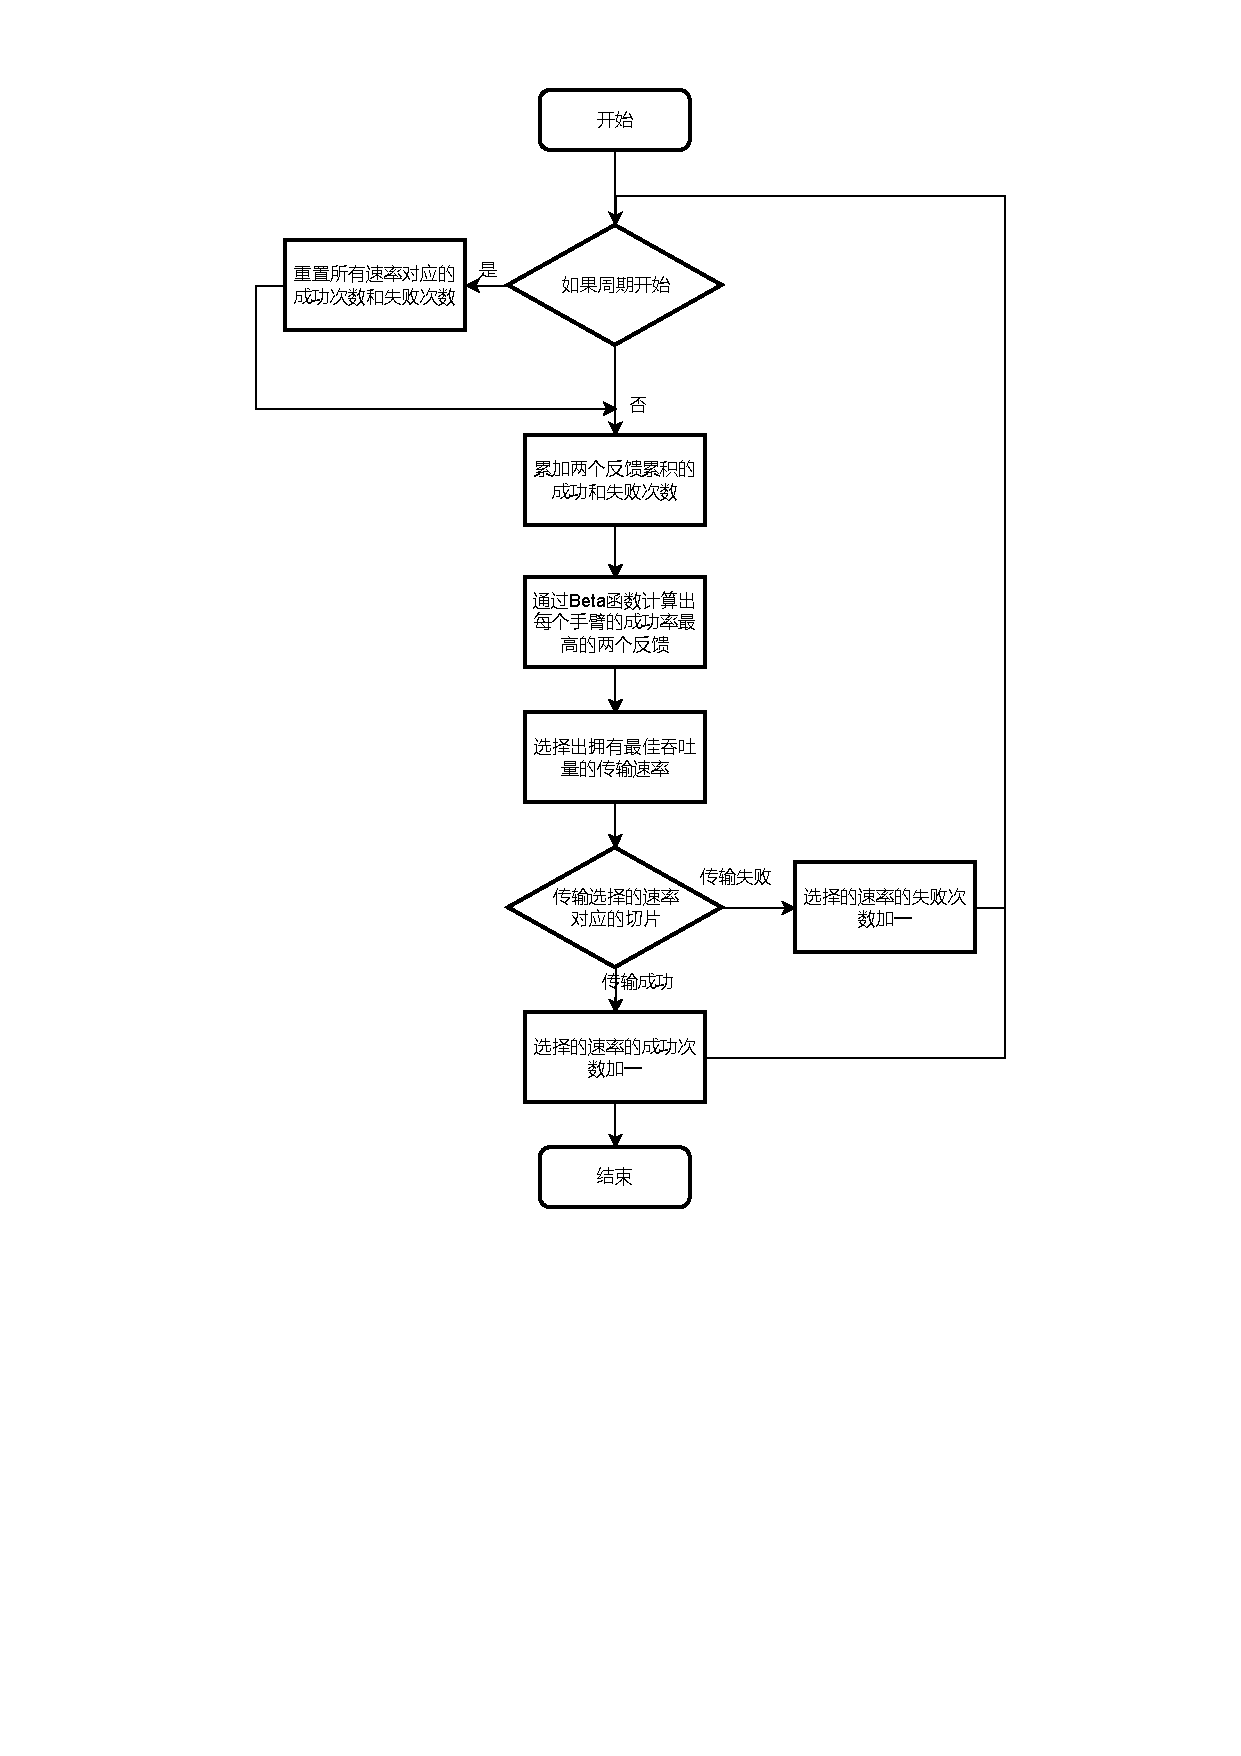
\includegraphics[width=0.8\textwidth]{figure/置零流程图.pdf}
	\caption{周期性重置Thompson Sampling算法流程图}
	\label{置零流程图}
\end{figure}

\section{基于折扣的Thompson Sampling算法}
在一个周期改变的信道中,我们可以想象越是时间久的数据是对当前的速度选择决策越是不重要,那么我们可以使用折扣系数来对不同的时间的成功次数和失败次数赋予不同的权重。的在基于折扣的Thompson Sampling算法中,一个臂所对应的成功次数或者失败次数并不是简单的相加,而是使用折扣系数对累积的数据赋予不同的权重。因此在算法中我们使用一个数组存储所有的数据。越早的数据权重越小,越近的数据权重越大。折扣系数范围在0~1之间。每一次实验结果以元组$\{1,2\}$或$\{0,1\}$方式存储,其中前者表示成功,后者表示失败。比如现在队列大小为5,队列存储的数据为$\{1,0\},\{0,1\},\{1,0\},\{0,1\},\{1,0\}$,折扣系数为0.9,那么输出的结果是$\{1*0.9^5+0*0.9^4+1*0.9^3+0*0.9^2+1*0.9^1,0*0.9^5+1*0.9^4+0*0.9^3+1*0.9^2+0*0.9^1\} = \{2.219,1.466\}$。
\begin{algorithm}[h]
	\ForEach{rate $r_{n},n = 1,2,...,N$}{
		$S_{n}^{(1)} \gets 0 \text { and } F_{n}^{(1)} \gets 0$
		
	}
	初始化空的数组$VEC$,
	\ForEach{$t = 1,2,...,T$}{
		\ForEach{rate $r_{n},n = 1,2,...,N$}{
			画出 $\alpha_{n}(t) \sim \operatorname{Beta}\left(S_{n}^{(1)}+1, F_{n}^{(1)}+1\right)^{2}$
			
			// 从数组中取出所有的数据,按照解释所演示的方法一样进行折扣计算并累加
			获得的折扣累加结果$\{S_{n}^{(2)}, F_{n}^{(2)}\}$
			
			画出 $\beta_{n}(t) \sim \operatorname{Beta}\left(S_{n}^{(2)}+1, F_{n}^{(2)}+1\right)^{2}$
			
		}
		选择满足下列条件的rate $r_{I(t)}$
		\begin{equation*}
			I(t)=\underset{n=1,2, \ldots, N}{\arg \max } r_{n} \alpha_{n}(t) \cdot \beta_{n}(t)
		\end{equation*}
	
		观察随机预测结果$X_{I(t)}(t)$和随机传输结果$Y_{I(t)}(t)$
		
		\If{$X_{I(t)}(t) = 1$}{
			$S_{n}^{(1)} \gets S_{n}^{(1)} + 1$
		}
		\Else{
			$F_{n}^{(1)} \gets F_{n}^{(1)} + 1$
		}
		\If{$Y_{I(t)}(t) = 1$}{
			把$\{1,0\}$压入$VEC$
		}
		\Else{
			把$\{0,1\}$压入$VEC$
		}		
	}
	\caption{\textbf{基于折扣的Thompson Sampling算法}}
	\label{sgd}
\end{algorithm}

由\ref{折扣流程图}可知基于折扣的Thompson Sampling算法重点在于计算累加值时需要先对历史数据进行折扣后再累加。

\begin{figure}[h]
	\centering
	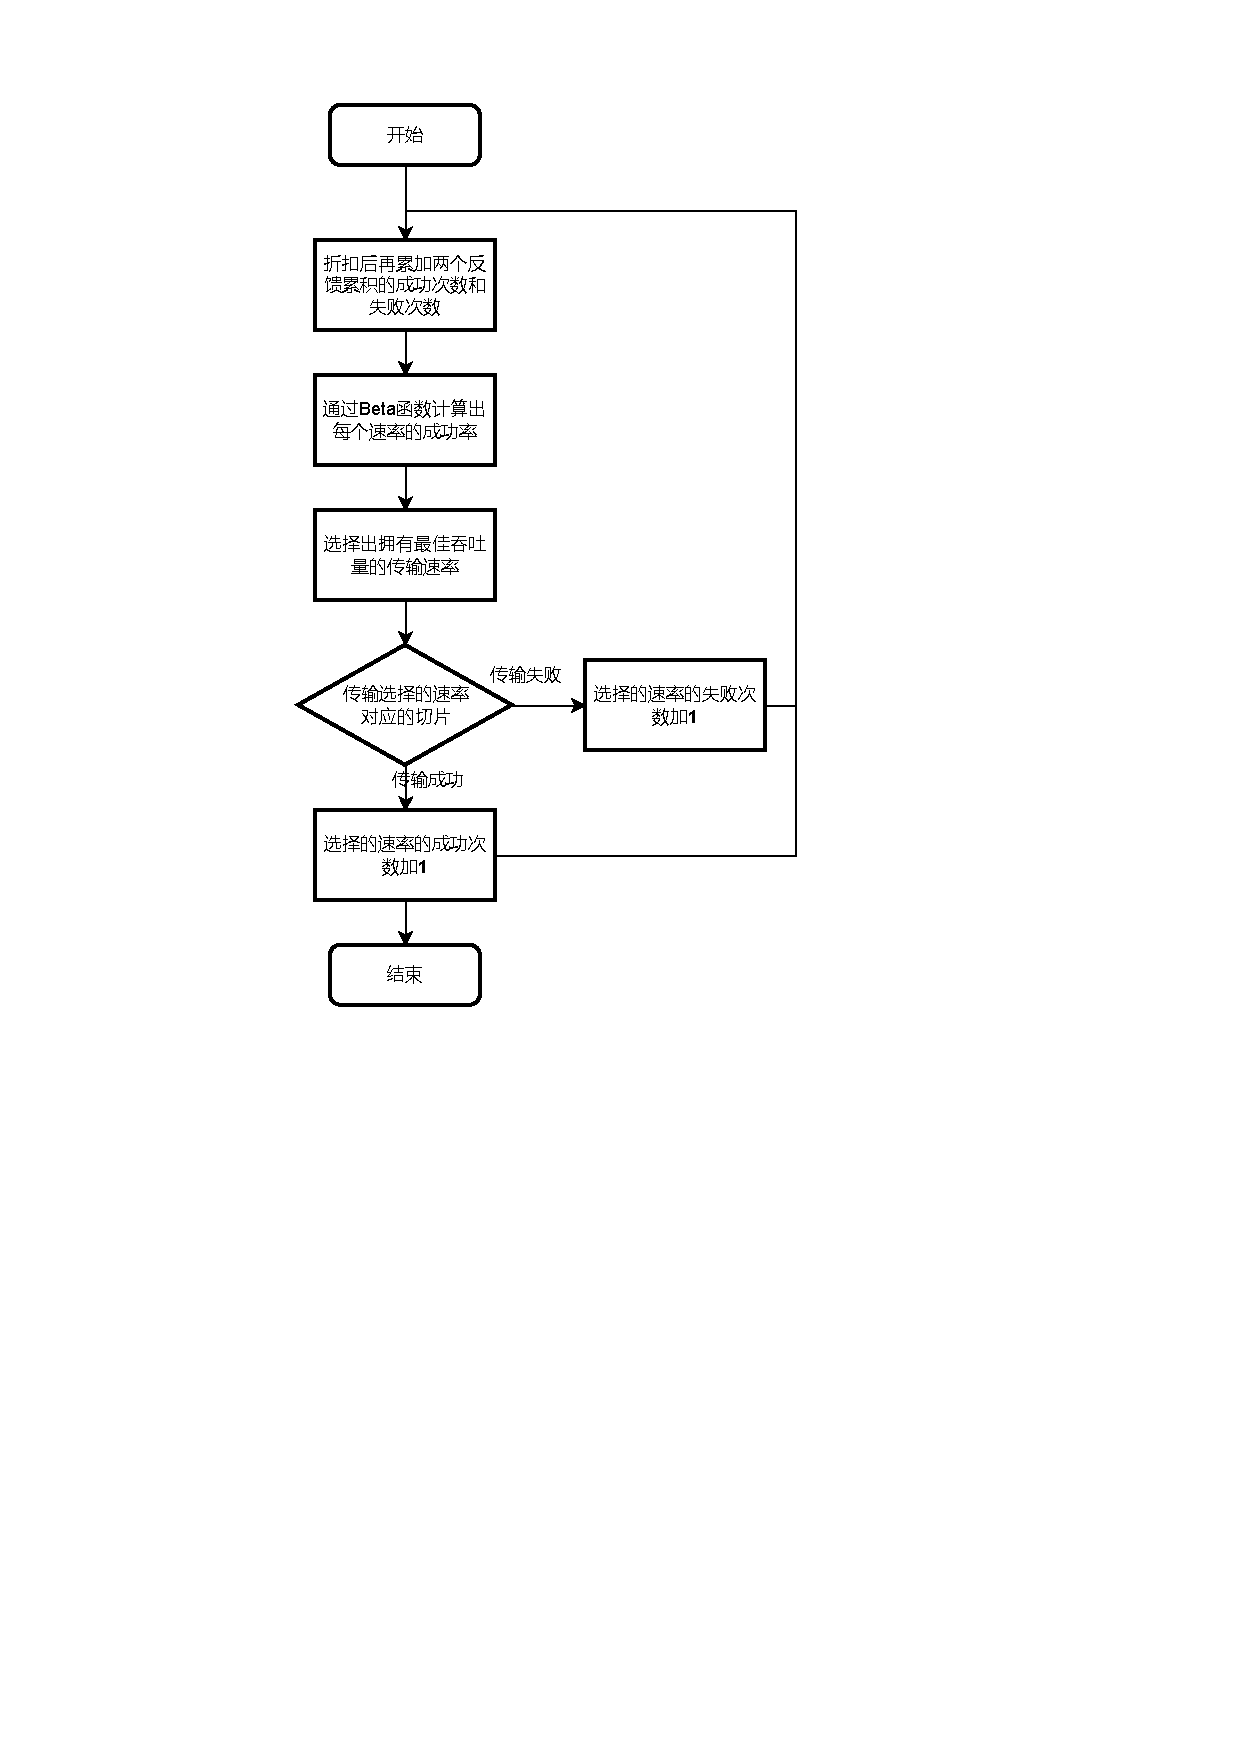
\includegraphics[width=0.8\textwidth]{figure/折扣流程图.pdf}
	\caption{基于折扣的Thompson Sampling算法}
	\label{折扣流程图}
\end{figure}

\section{基于滑动窗口的Thompson Sampling算法}
不管怎么说,基于折扣的Thompson Sampling算法中,过去的不重要的数据还是对当前的决策有影响,那么我们可以用一个滑动窗口把最近的数据划出来,其他的数据丢弃。这么做的另一个好处是不需要一直存储着所有数据。当数据量过大时,基于折扣的Thompson Sampling算法在每个时隙都需要重新计算折扣累加值,这相当的耗费时间。在基于滑动窗口的Thompson Sampling算法中,我们维护一个固定容量的窗口,窗口的容量是指能存储的试验次数。这个窗口里面包含了所有手臂的实验结果。每一次实验结果以元组$\{1,k\}$或$\{0,k\}$方式存储,其中前者表示实验结果,如果是1表示成功,0表示失败。,后者表示这是第k个手臂的实验结果。当存储的实验结果达到窗口容量时,每当存储新的结果时,需要把最早存储的结果从窗口中弹出来。获取某个手臂的累加结果时需要遍历滑动窗口来计算。
\begin{algorithm}[h]
	初始化滑动窗口 $SW$
	
	\ForEach{rate $r_{n},n = 1,2,...,N$}{
		$S_{n}^{(1)} \gets 0 \text { and } F_{n}^{(1)} \gets 0$
		
	}
	\ForEach{$t = 1,2,...,T$}{
		\ForEach{rate $r_{n},n = 1,2,...,N$}{
			画出 $\alpha_{n}(t) \sim \operatorname{Beta}\left(S_{n}^{(1)}, F_{n}^{(1)}\right)^{2}$
			
			// 累加滑动窗口中所有的值
			从滑动窗口$SW$中计算得到$r_{n}$的累加结果$S_{n}^{(2)}$和$F_{n}^{(2)}$
			
			画出 $\beta_{n}(t) \sim \operatorname{Beta}\left(S_{n}^{(2)}, F_{n}^{(2)}\right)^{2}$
			
		}
		选择满足下列条件的rate $r_{I(t)}$
		\begin{equation*}
			I(t)=\underset{n=1,2, \ldots, N}{\arg \max } r_{n} \alpha_{n}(t) \cdot \beta_{n}(t)
		\end{equation*}
	
		观察随机预测结果$X_{I(t)}(t)$和随机传输结果$Y_{I(t)}(t)$
		
		\If{$X_{I(t)}(t) = 1$}{
			$S_{n}^{(1)} \gets S_{n}^{(1)} + 1$
		}
		\Else{
			$F_{n}^{(1)} \gets F_{n}^{(1)} + 1$
		}
		\If{$Y_{I(t)}(t) = 1$}{
			把$\{1,0\}$压入$SW$
		}
		\Else{
			把$\{0,1\}$压入$SW$
		}
		\If{滑动窗口$SW$大小超过容量}{
			弹出最早的数据
		}
	}
	\caption{\textbf{基于滑动窗口的Thompson Sampling算法}}
	\label{sgd}
\end{algorithm}

由\ref{滑动流程图}可知基于滑动窗口的Thompson Sampling算法重点在于积累的数据大小有一个局限,如果超出局限需要先弹出最早的数据再存储。

\begin{figure}[h]
	\centering
	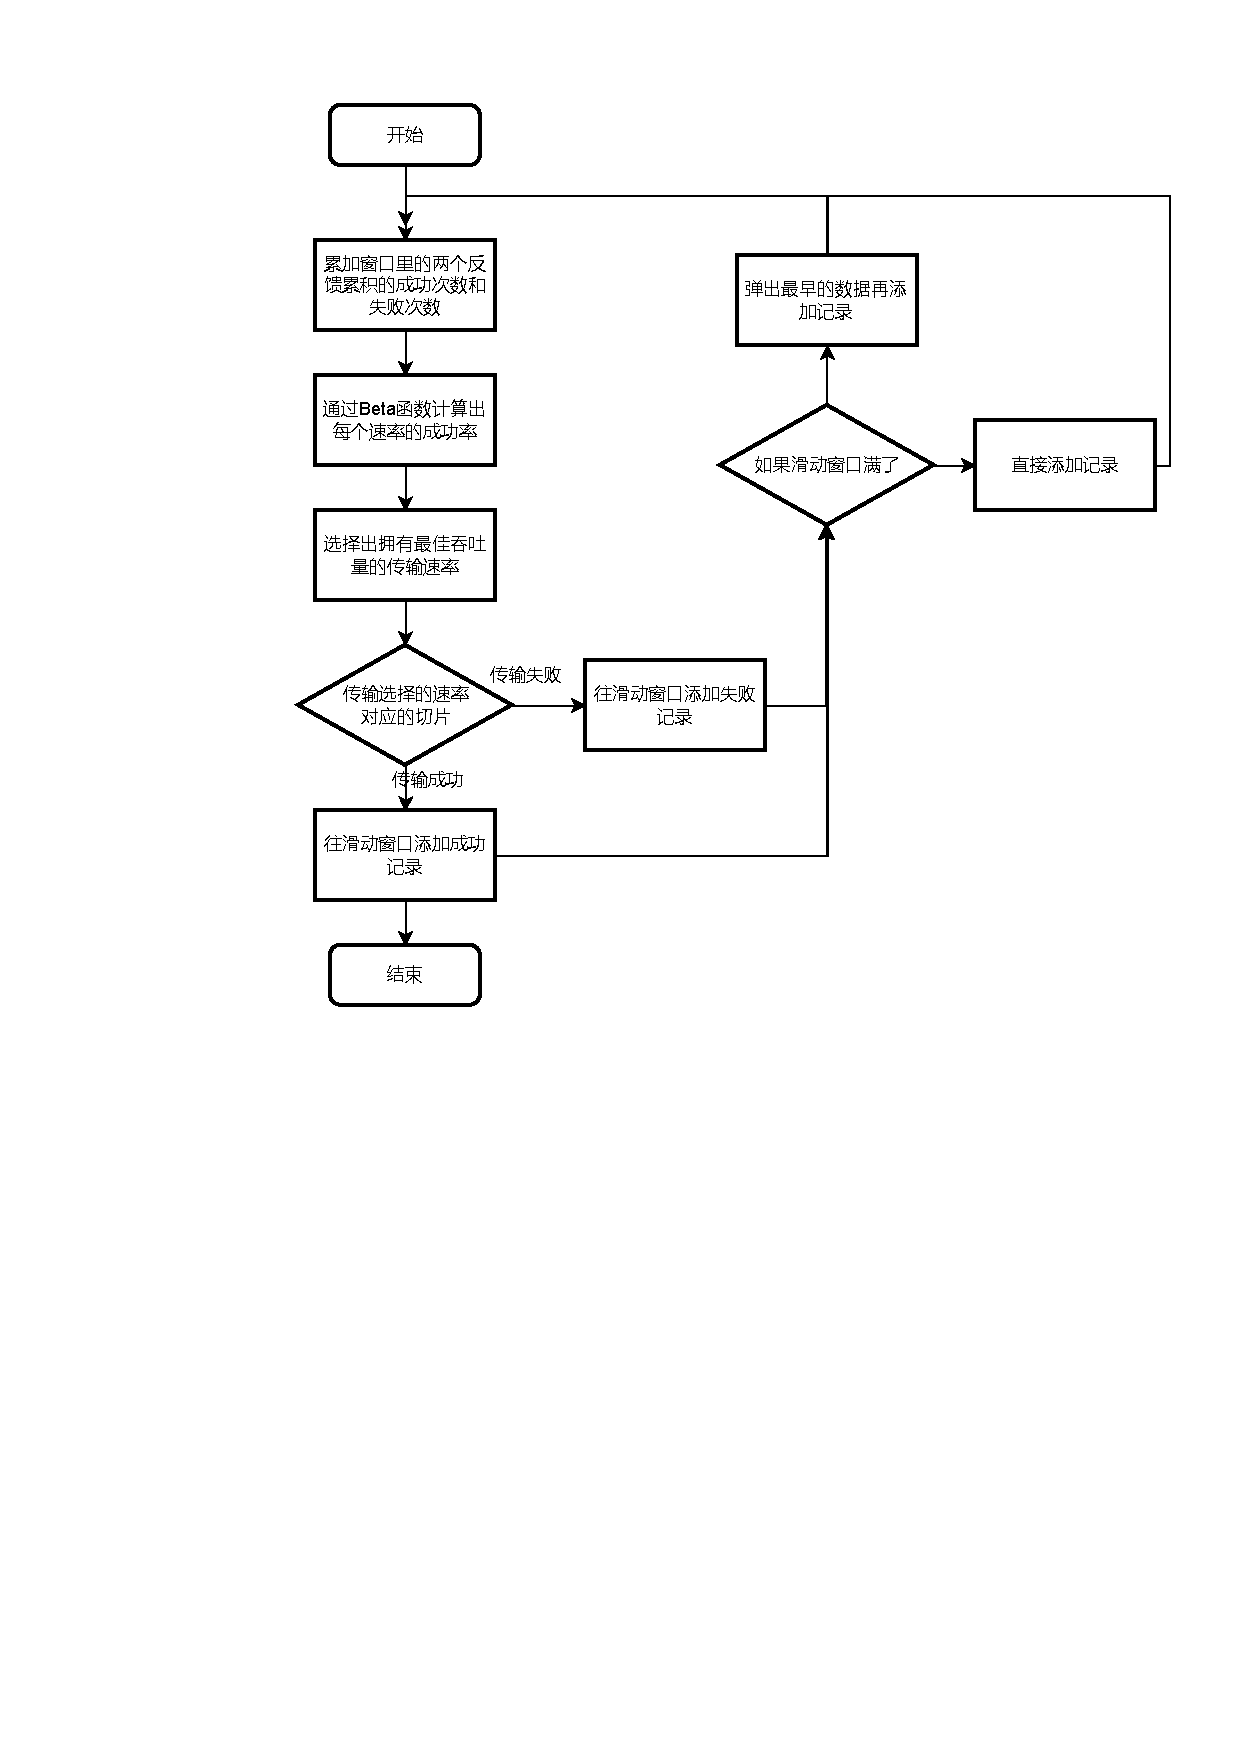
\includegraphics[width=0.8\textwidth]{figure/滑动流程图.pdf}
	\caption{基于滑动窗口的Thompson Sampling算法}
	\label{滑动流程图}
\end{figure}

\section{基于增加次数的滑动窗口Thompson Sampling算法}
在基于滑动窗口的Thompson Sampling算法中,我们或许会碰到这种问题:周期发生变化时,算法还是不能快速反应过来选择出正确的手臂(ARM)。为什么呢?因为在周期发生变化的时候,滑动窗口里面可能大部分数据都是上一个周期的没用数据。如果我们在滑动窗口里面增加两个规则:(1)如果选择的速度超过了阈值(比如占用了滑动窗口容量的一半或者更多),而且这个速度在传输过程中失败了,那么我们不再是只增加一次失败次数$F_{n}^{(1)}(t)$,而是增加更多。因为出现这种可能性时往往表示信道容量发生变化了。(2)如果选择的手臂(ARM)在传输过程中成功了而且有其他手臂超过了阈值(比如占用了滑动窗口容量的一半或者更多),那么我们会给这个手臂对应的成功次数增加更多。在这个算法中,滑动窗口将存储每一次成功的“次数”和失败的“次数”,因此压入滑动窗口的值的形式为$[arm_index, success_number, fail_number]$。

\begin{algorithm}[h]
	初始化滑动窗口 $SW$
	
	\ForEach{rate $r_{n},n = 1,2,...,N$}{
		$S_{n}^{(1)} \gets 0 \text { and } F_{n}^{(1)} \gets 0$
		
	}
	设置阈值$threshold$
	\ForEach{$t = 1,2,...,T$}{
		\ForEach{rate $r_{n},n = 1,2,...,N$}{
			画出 $\alpha_{n}(t) \sim \operatorname{Beta}\left(S_{n}^{(1)}, F_{n}^{(1)}\right)^{2}$
			
			从滑动窗口$SW$中计算得到$r_{n}$的累加结果$S_{n}^{(2)}$和$F_{n}^{(2)}$\\
			画出 $\beta_{n}(t) \sim \operatorname{Beta}\left(S_{n}^{(2)}, F_{n}^{(2)}\right)^{2}$
			
		}
		选择满足下列条件的rate $r_{I(t)}$
		\begin{equation*}
			I(t)=\underset{n=1,2, \ldots, N}{\arg \max } r_{n} \alpha_{n}(t) \cdot \beta_{n}(t)
		\end{equation*}
	
		观察随机预测结果$X_{I(t)}(t)$和随机传输结果$Y_{I(t)}(t)$
		
		\If{$X_{I(t)}(t) = 1$}{
			$S_{n}^{(1)} \gets S_{n}^{(1)} + 1$
		}
		\Else{
			$F_{n}^{(1)} \gets F_{n}^{(1)} + 1$
		}
		// 如果窗口里面有速度对应的成功数量大于阈值, 则增加成功的次数
		
		\If{$Y_{I(t)}(t) = 1$ AND 有非$I(t)$的$threshold \geq armCounts $} {
			
			把$\{I(t), add_number, 0\}$压入$SW$
			
		}
	
		// 如果窗口里面选择的速度$r_{n}$对应的成功数量大于阈值, 则增加失败的次数
		
		\If{$Y_{I(t)}(t) = 0$ AND $I(t)$的$threshold \geq armCounts$}{
			
			把$\{I(t), 0, sub_number\}$压入$SW$
			
		}
	
		\If{滑动窗口$SW$大小超过容量}{
			
			弹出最早的数据
			
		}
	
	}

	\caption{\textbf{基于增加次数的Thompson Sampling算法}}
	\label{sgd}
\end{algorithm}

由\ref{增加次数流程图}可知基于增加次数的滑动窗口Thompson Sampling算法重点在于每次累积的数据不止一个,这需要根据信道特性进行设置,以便获取最佳吞吐量。

\begin{figure}[h]
	\centering
	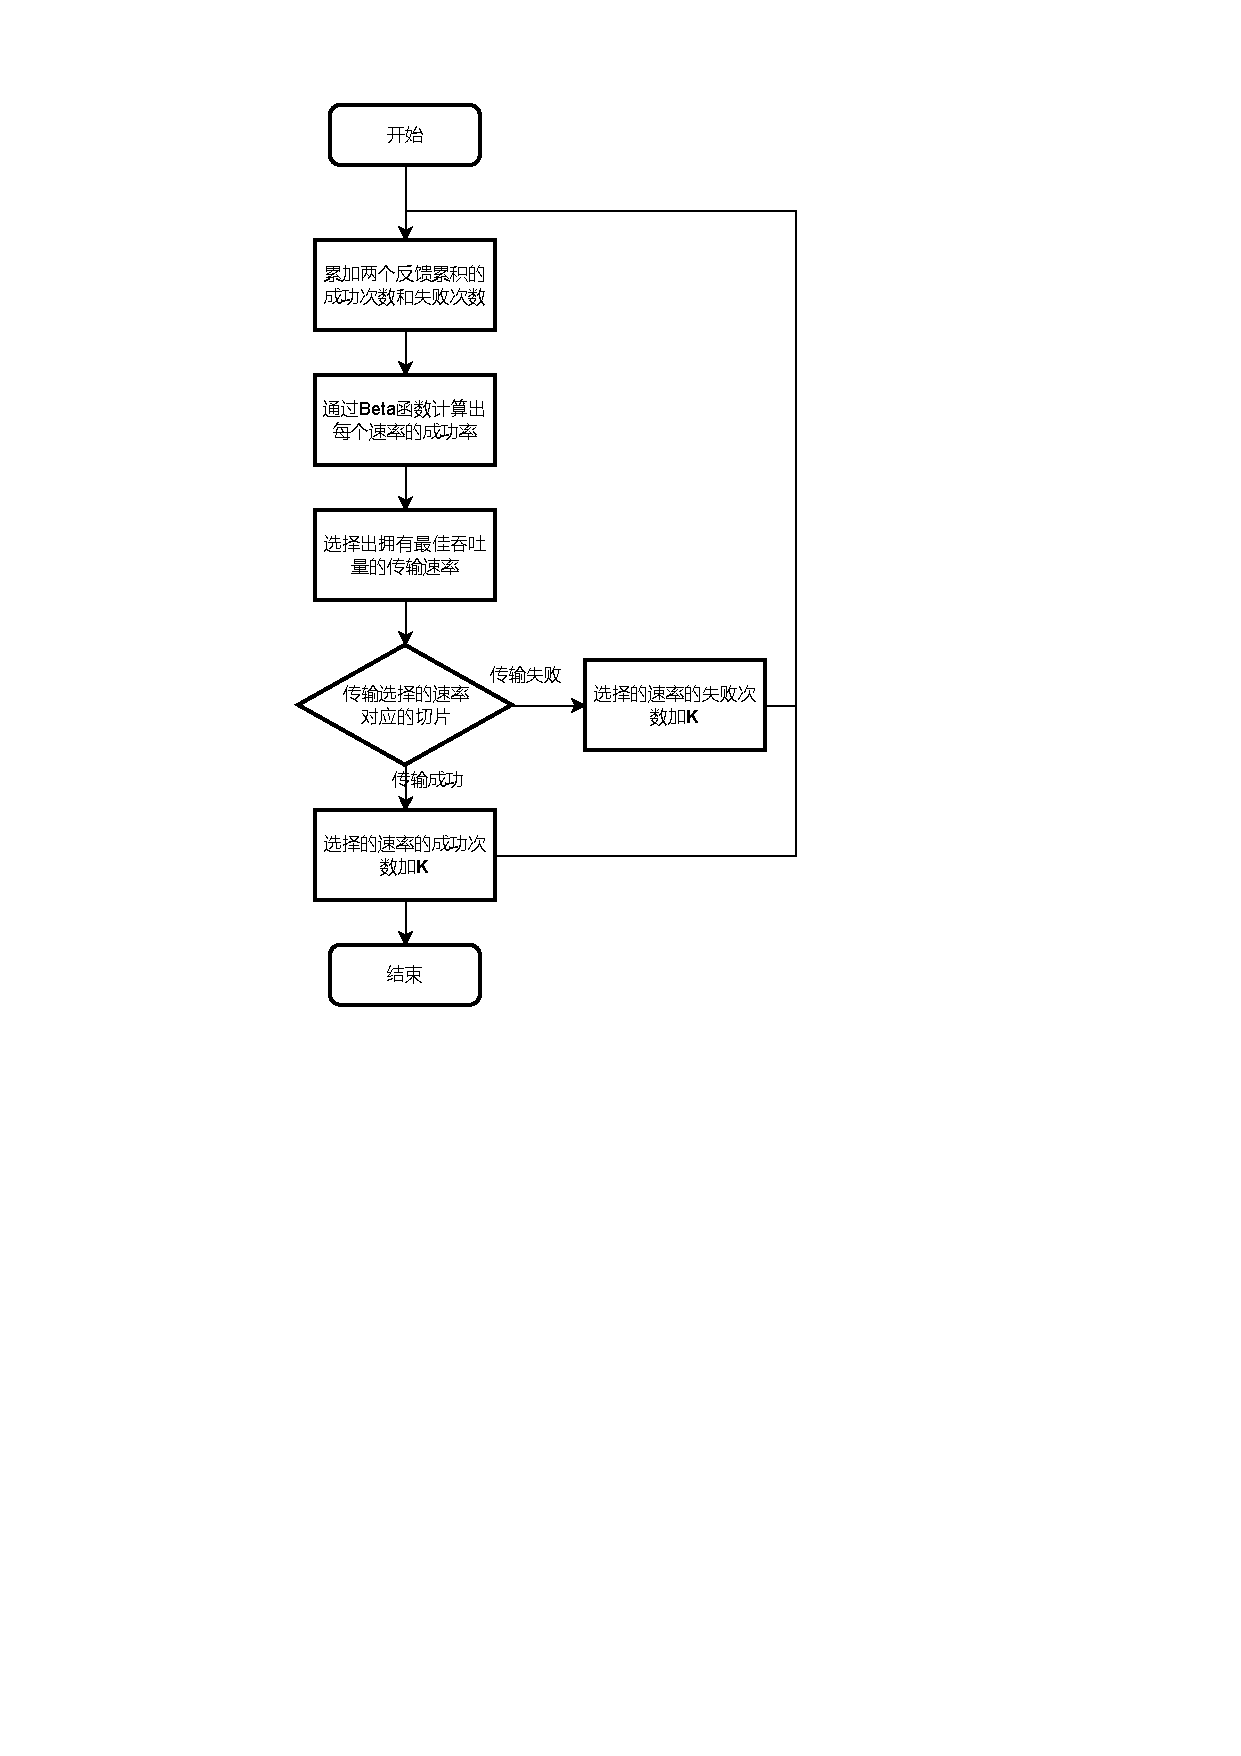
\includegraphics[width=0.8\textwidth]{figure/增加次数流程图.pdf}
	\caption{基于增加次数的滑动窗口Thompson Sampling算法}
	\label{增加次数流程图}
\end{figure}

\section{基于折扣、增加次数和滑动窗口的Thompson Sampling算法}
在上述的除了周期性重置Thompson Sampling算法外,我们是否可以把所有的有点结合起来呢?当然可以,这就是基于折扣、增加次数和滑动窗口的Thompson Sampling算法。
\begin{algorithm}[h]
	初始化滑动窗口 $SW$
	\ForEach{rate $r_{n},n = 1,2,...,N$}{
		$S_{n}^{(1)} \gets 0 \text { and } F_{n}^{(1)} \gets 0$
	}
	设置阈值$threshold$
	\ForEach{$t = 1,2,...,T$}{
		\ForEach{rate $r_{n},n = 1,2,...,N$}{
			画出 $\alpha_{n}(t) \sim \operatorname{Beta}\left(S_{n}^{(1)}, F_{n}^{(1)}\right)^{2}$\\
			从滑动窗口$SW$中计算得到$r_{n}$的折扣累加结果$S_{n}^{(2)}$和$F_{n}^{(2)}$\\
			画出 $\beta_{n}(t) \sim \operatorname{Beta}\left(S_{n}^{(2)}, F_{n}^{(2)}\right)^{2}$\\
		}
		选择满足下列条件的rate $r_{I(t)}$
		\begin{equation*}
			I(t)=\underset{n=1,2, \ldots, N}{\arg \max } r_{n} \alpha_{n}(t) \cdot \beta_{n}(t)
		\end{equation*}\\
		观察随机预测结果$X_{I(t)}(t)$和随机传输结果$Y_{I(t)}(t)$
		
		\If{$X_{I(t)}(t) = 1$}{
			$S_{n}^{(1)} \gets S_{n}^{(1)} + 1$
		}
		\Else{
			$F_{n}^{(1)} \gets F_{n}^{(1)} + 1$
		}
		\If{$Y_{I(t)}(t) = 1$ AND 有非$I(t)$的$armCounts \geq threshold $} {
			
			把$\{I(t), add_number, 0\}$压入$SW$
			
		}
	
		\If{$Y_{I(t)}(t) = 0$ AND $I(t)$的$armCounts \geq threshold$}{
			
			把$\{I(t), 0, sub_number\}$压入$SW$
			
		}
	
		\If{滑动窗口$SW$大小超过容量}{
			弹出最早的数据\\
		}
	}
	\caption{\textbf{基于滑动窗口的Thompson Sampling算法}}
	\label{sgd}
\end{algorithm}

\section{本章小结}
在周期信道中,我们基于Thompson Sampling算法又开发出五个新的算法,分别周期性重置Thompson Sampling算法、基于折扣的Thompson Sampling算法、基于滑动窗口的Thompson Sampling算法为和基于折扣滑动窗口的Thompson Sampling算法。这些算法是我们根据周期性容量变化的信道的特点而开发的,那么这些算法是否有效呢?在本文的下一章将通过仿真实验来验证。


